\chapter{Introdução}
\label{cha:introducao}

Para efeitos didáticos, podemos dividir as disciplinas do curso de Sistemas de Informação em três ou quatro núcleos: 1) as matérias de matemática, 2) as matérias de gestão e 3) as matérias de ciência da computação que podemos subdividir em matérias teóricas e matérias de sistemas.
Originalmente esta disciplina que hoje chamamos de ``Introdução à Programação'' era chamada de ``Introdução à Ciência da Computação'' e tinha como objetivo introduzir os ingressantes aos temas que seriam tratados no núcleo 3.
Imagino que a mudança de nome teve a intenção de deixar mais claro que o que se espera dos estudantes ao final do curso é que eles tenham ``aprendido a programar'', como se diz de maneira informal, ou ao menos tenham sido iniciado nessa arte.
Quando ofereci esta disciplina pela primeira vez, porém, julguei útil tentar reter um pouco da ideia original do curso, a saber, introduzir alguns dos conceitos com os quais vocês, estudantes ingressantes do curso de Sistemas de Informação, irão se deparar ao longo do curso.
Pretendo manter esse espírito sem prejuízo, porém, de cobrir todo conteúdo que se espera de um curso de Introdução à Programação.

Aprender a programar se assemelha um pouco ao processo de aprender uma nova língua.
Cabe ao professor passar parte do novo léxico e os conceitos da nova gramática, mas essa aproximação conceitual ao objeto de estudos de nada adianta sem o exercício prático da fala, da escuta e da escrita.
Por esse motivo, e porque a experiência mostrou a eficácia do modelo, optamos por intercalar neste curso aulas conceituais e aulas práticas no laboratório.
O enfoque desta apostila é na parte conceitual do curso, mas incluímos no final de quase todo capítulo sugestões de exercícios práticos.
Os exercícios, portanto, não são opcionais e exigem dedicação dos estudantes, bem como o acompanhamento atento do docente e seu(s) monitore(s).

Comecemos nossa apostila, então, tratando do conceito fundamental: {\em computação}.
A maneira clássica de apresentar a história da computação, divide-a em duas trajetórias progressivas e relativamente independentes \cite{}.
Acreditamos que essa apresentação é simplista, mas serve bem aos propósitos desta introdução.

A primeira trajetória centra sua atenção no artefato, o {\em computador}.
Ela começa com a invenção do ábaco em tempos imemoráveis e passa por uma série de tentativas de construir o que hoje chamaríamos de máquinas de calcular, passa pelas máquinas Hollerith até chegar no EDVAC, no ENIAC, no Colossus, nos microcomputadores e assim por diante.
A segunda, a que nos interessa, centra sua atenção no conceito, a {\em computação}.
Essa história começa com ideias de filósofos como Leibniz que no século XVII imaginou que o limite do método analítico de raciocínio era sua automatização.
Essa ideia atravessou os séculos e teve seu período áureo no começo do século XX quando uma série de pesquisadores brilhantes se debruçaram sobre o problema de formalizar toda a matemática.
Esse esforço eventualmente esbarrou no seguinte problema: seria possível automatizar o processo de construção de provas matemáticas?
O personagem principal da nossa história, o matemático inglês Allan Turing, entendeu que isso não era sempre possível.
Para mostrar isso, porém, ele precisou definir de maneira convincente o que significa um procedimento ser automatizável.

Outros matemáticos daquela época -- notavelmente Alonzo Church, Kurt Gödel e Emilie Post -- haviam proposto modelos alternativos que não foram suficientemente convincentes.
Uma das novidade do modelo de Turing, hoje conhecido como ``Máquinas de Turing'', era a possibilidade de se construir uma ``Máquina Universal''.
Ou seja, uma máquina capaz de reproduzir o comportamento de qualquer outra Máquina de Turing.

Toda esta história será contada com muito mais detalhes no curso de {\em Introdução à Teoria da Computação}.
Talvez o resultado principal do curso será mostrar, como Turing o fez nos anos 30, que existem problemas matemáticos que não podem ser resolvidos de maneira automática.
Para os propósitos destas notas, porém, o que queremos reter é algo mais simples:

\begin{quote}
  Um {\em computador} é uma máquina programável de processamento de dados capaz de simular qualaquer outra máquina de processamento de dados.
\end{quote}

Ou seja, um computador não se confunde com uma máquina de calcular ou com as máquinas Hollerith que era construídas com um propósito específico.
Um computador pode ser programado para fazer qualquer coisa, ou melhor, qualquer coisa que seja possível automatizar.

Portanto, conceitualmente um computador é uma máquina programável universal.
Essa ideia de Turing se realiza em máquina concreta por meio de uma arquitetura.
No curso de {\em Arquitetura de Computadores} vocês estudarão esse tema a fundo.
Aqui vamos apresentar apenas as ideias principais da chamada {\em arquitetura de Von Neumann}.

A característica marcante dessa arquitetura é a separação entre uma unidade de processamento (CPU) -- que contém uma unidade de controle, uma unidade lógica e registradores -- e uma unidade de memória (Figura \ref{fig:von-neumann}).

\begin{figure}[htbp]
  \centering
  \includegraphics[width=.5\textwidth]{imagens/von-neumann.jpg}
  \caption{Arquitetura de Von Neumann}
  \label{fig:von-neumann}
\end{figure}

A CPU é uma máquina universal capaz de executar programas armazenados na unidade de memória.

Podemos agora dizer com todas as letras que o objetivo desta disciplina é introduzir os estudantes à arte de programar essas máquinas chamadas computadores.
Para tanto precisaremos aprender uma {\em linguagem de programação}.

Antes de começarmos a falar de linguagens, porém, convém dar um passo atrás e entender o que exatamente queremos programar.
Para tanto será útil um outro conceito central para o curso: {\em algoritmo}.

\begin{quote}
  Um {\em algoritmo} é uma sequência de instruções inequívocas a serem executadas em passos discreto -- ou seja, um de cada vez.
  Em geral um algoritmo pode partir de um valor inicial que será chamado de {\em entrada} e sua execução pode eventualmente parar e devolver um valor chamado de {\em saída}.
\end{quote}

Algoritmos serão o objeto de estudos no curso de {\em Introdução à Análise de Algoritmos}.
Por ora, nos interessa apenas concretizar a ideia com alguns exemplos.

\begin{example}{Algoritmo de Euclides}
  \label{ex:euclides}

  \noindent
  {\bf Entrada:} Dois inteiros $a$ e $b$ tais que $a \geq b$\\
  {\bf Saída:} O maior divisor comum entre $a$ e $b$
  \begin{enumerate}
  \item Calcule o resto $r$ da divisão de $a$ por $b$
  \item Chame $b$ de $a$ e $r$ de $b$
  \item Se $b \neq 0$ volte para o passo 1
  \item Se $b = 0$ para e devolva $a$
  \end{enumerate}

  \noindent
  {\bf Simulação:}
  \begin{itemize}
  \item $a = 42$, $b = 24$ e $r = 18$
  \item $a = 24$, $b = 18$ e $r = 6$
  \item $a = 18$, $b = 6$ e $r = 0$
  \item $a = 6$, $b = 0$ e devolve $6$
  \end{itemize}
\end{example}

O Exemplo \ref{ex:euclides} mostra um procedimento para determinar o máximo divisor comum entre dois números inteiros conhecido como {\em Algoritmo de Euclides}.
Esse algoritmo está descrito no livro {\em Elementos} escrito por Euclides por volta do ano 300 a.c.
Não é trivial verificar que ele é {\em correto}, ou seja, que para quaisquer duas entradas $a$ e $b$ satisfazendo a condição $a \geq b$ a saída será o máximo divisor comum entre $a$ e $b$.
Uma técnica para demonstrar que um algoritmo é correto será apresentada no curso de {\em Introdução à Análise de Algoritmos}.
Nos interessa, por enquanto, apenas a definição:

\begin{quote}
  Um algoritmo é {\em correto} se para toda entrada válida ele devolve a saída esperada.
\end{quote}

Note que a definição que demos de algoritmo não exige que ele necessariamente pare em algum momento.
De fato, podemos pensar exemplos de algoritmos que satisfazem nossa definição, mas que é difícil de mostrar se ele chega a um fim para todas as entradas.
Considere o seguinte exemplo:

\begin{example}{Algoritmo $3N+1$}
  \label{ex:euclides}

  \noindent
  {\bf Entrada:} Um número natural $N$
  \begin{enumerate}
  \item Se $N$ é para coloque $\frac{N}{2}$ em $N$ e repita
  \item Se $N$ é ímpar e $N \neq 1$ coloque $3N+1$ em $N$ e volte para o passo 1
  \item Se $N = 1$ pare
  \end{enumerate}

  \noindent
  {\bf Simulação:}
  \begin{itemize}
  \item $N = 42$
  \item $N = 24$
  \item $N = 64$
  \item $N = 32$
  \item $N = 16$
  \item $N = 8$
  \item $N = 4$
  \item $N = 2$
  \item $N = 1$
  \end{itemize}
\end{example}

Até o presente momento não conhecemos uma demonstração matemática de que o algoritmo $3N+1$ termina para todas as entradas ou se existe alguma entrada para o qual ele nunca termina -- neste segundo caso dizemos que a simulação entra em {\em loop infinito}.
Como já chamamos a atenção, porém, nossa definição de algoritmo não depende disso.

Uma {\em linguagem de programação} materializa um algoritmo em um programa.
Ou inversamente, um {\em algoritmo} abstrai a linguagem de um programa.

\begin{center}
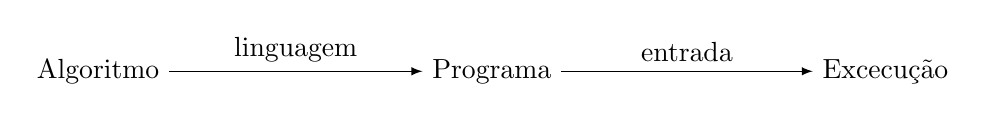
\begin{tikzpicture}[node distance=2cm,auto,>=latex]
\node (algo) {Algoritmo};
\node (prog) at (5,0) {Programa};
\node (exec) at (10,0) {Excecução};
\draw[->] (algo) -> node[above]{linguagem} (prog);
\draw[->] (prog) -> node[above]{entrada} (exec);
\end{tikzpicture}
\end{center}

Como qualquer linguagem, uma linguagem de programação possui:
\begin{itemize}
\item um conjunto de palavras reservadas ({\em léxico}), 
\item um conjunto de regras que definem a estrutura de sentenças a partir do léxico ({\em gramática} ou {\em sintaxe}) e
\item um conjunto de instruções que determinam como devem ser interpretadas as sentenças ({\em semântica}).
\end{itemize}

Considere como exemplo o seguinte pequeno trecho de um código escrito na linguagem Java:

\begin{lstlisting}
if(c > 0){
  c = c + 1;
}
\end{lstlisting}

O termo {\tt if} é uma palavra reservada e, portanto, faz parte do seu léxico, bem como os símbolos de chaves, parênteses e ponto e vírgula.
A estrutura -- sintaxe -- pode ser descrita da seguinte forma:

\begin{lstlisting}
if(<cond.>){
  <bloco>
}
\end{lstlisting}

Para ser mais preciso, precisaríamos descrever a sintaxe de {\tt <cond.>} e de {\tt <bloco>}, mas vamos para por aqui.
Por fim, a semântica deste comando determina que caso a condição {\tt <cond.>} seja satisfeita, o bloco {\tt <bloco>} será executado.

Alguns cursos de computação oferecem a disciplina {\em Linguagens de Programação} que explora a fundo as opções sintáticas e a semânticas de diversas linguagens.
Com exceção da já mencionada disciplina de Arquitetura, em todos os demais disciplinas usaremos linguagens de alto nível, ou seja, linguagens que não são interpretadas diretamente pela CPU.
Algumas linguagens de programação como C, que vocês devem ter contato nas disciplinas de {\em Estrutura de Dados}, possuem o que chamamos de um compilador.
Alguns cursos de computação oferecem a disciplina de {\em Compiladores} que trata exclusivamente deste tema.

\begin{quote}
  Um {\em compilador} é um programa que traduz um programa de uma linguagem para outra.
\end{quote}

No caso do compilador de C, o programa escrito em C é traduzido para uma linguagem a ser diretamente executada pela CPU.

\begin{center}
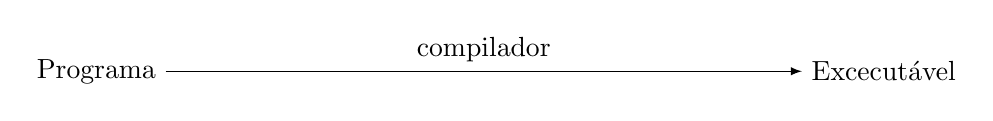
\begin{tikzpicture}[node distance=2cm,auto,>=latex]
\node (prog) {Programa};
\node (exec) at (10,0) {Excecutável};
\draw[->] (prog) -> node[above]{compilador} (exec);
\end{tikzpicture}
\end{center}

Outras linguagens, como o Python, seguem uma abordagem diferente.
Para executar um programa em Python é preciso de um programa chamado de {\em interpretador} que interpreta suas instruções.

\begin{center}
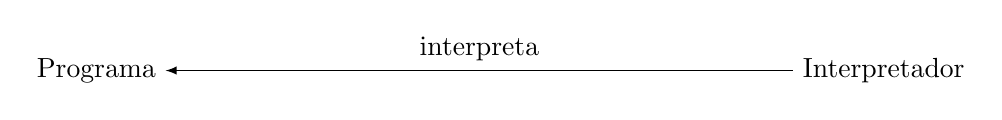
\begin{tikzpicture}[node distance=2cm,auto,>=latex]
\node (prog) {Programa};
\node (int) at (10,0) {Interpretador};
\draw[<-] (prog) -- node[above]{interpreta} (int);
\end{tikzpicture}
\end{center}


Nesta disciplina nos centraremos em uma linguagem específica, a última versão do Java.
Programas escritos na linguagem Java combinam os dois paradigmas descritos acima numa tentativa de reter o melhor dos dois: a eficiência das linguagens compiladas e a capacidade das linguagem script de funcionarem em diferentes arquiteturas.
Um programa em Java precisa, então, ser compilados para uma linguagem intermediária chamada {\em Bytecode} que, por sua vez, é interpretada por um outro programa também chamado Java\footnote{Eu sei, é um pouco confuso mesmo}.

\begin{center}
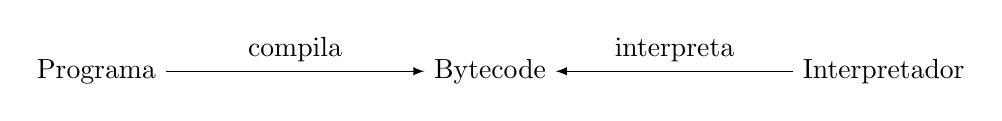
\begin{tikzpicture}[node distance=2cm,auto,>=latex]
\node (prog) {Programa};
\node (byte) at (5,0) {Bytecode};
\node (int) at (10,0) {Interpretador};
\draw[->] (prog) -- node[above]{compila} (byte);
\draw[<-] (byte) -- node[above]{interpreta} (int);
\end{tikzpicture}
\end{center}

Podemos então, finalmente escrever nosso primeiro programa:

\begin{lstlisting}
// Hello World
public class Hello{
  public static void main(String[] args){
    System.out.println("Ola Mundo");
  }
}
\end{lstlisting}

Aos poucos vamos destrinchando o que significa cada linha deste programa, por ora basta dizer que vamos escrevê-lo em um arquivo chamado {\tt Hello.java} que deve ser compilado para gerar um arquivo Bytecode chamado {\tt Hello.class} que pode finalmente ser interpretado.

\begin{center}
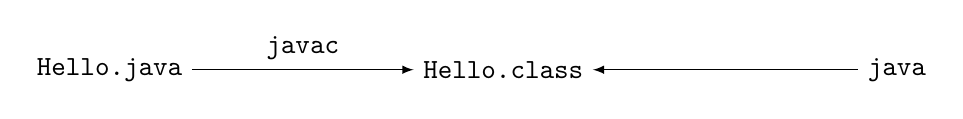
\begin{tikzpicture}[node distance=2cm,auto,>=latex]
\node (prog) {\tt Hello.java};
\node (byte) at (5,0) {\tt Hello.class};
\node (int) at (10,0) {\tt java};
\draw[->] (prog) -- node[above]{\tt javac} (byte);
\draw[<-] (byte) -- (int);
\end{tikzpicture}
\end{center}


% linguagem: léxico, sintaxe e semântica

% compilador - compiladores

% exemplos: C, python e Java